% !TEX root = ./pkArticle.tex
\mode*
\section{Elimination, Halbwertszeit}
\mode<all>
% !TEX root = ./pkArticle.tex
\mode*

\subsection{Elimination, Context sensitive Halbwertszeit}

Mit der {\it Halbwertszeit} (\HWZ) wird die Geschwindigkeit von (biologischen) Prozessen beschrieben. Beim radiokativen Zerfall ist die Aktivit�t nach einer \HWZ  
halbiert. Nach zwei \HWZ betr�gt die Aktivit�t noch die H�lfte der H�lfte d.h. ein Viertel.

Diese �berlegungen lassen sich nicht direkt auf den Konzentrationsabfall von Medikamenten �bertragen. Die einzelnen Umvertelungsprozesse k�nnen ebenfalls mit \HWZ beschrieben werden doch ist die Bedeutung nicht dieselbe wie beim radiokativen Zerfall. Deshalb soll die {\it Elimination} etwas allgemeiner betrachtet werden.

\begin{frame}
\frametitle{Elimination}
\begin{itemize}[<+->]
\item
Elimination aus K\"orper oder Elimination aus Blut?
\item
Konzentrationsabfall: Umverteilung und Metabolisierung
\item
Es kann aktive Metaboliten geben
\item
Fettl\"osliche Medikamente werden in Leber zu inaktiven, wasserl\"oslichen Metaboliten umgewandelt
\item
Ausscheidung der wasserl\"oslichen Substanzen durch Niere
\item
Pharmakokinetik {\bf{quantifiziert}} die Geschwindikeit der Elimination
\end{itemize}

\note<1>{

\begin{itemize}
\item
Elimination wird meist als \enquote{Kleinerwerden der Konzentration} des Medikamentes im Blut quantifiziert!
\item
Meist denkt man dabei an die Elimination des Medikamentes aus dem \enquote{Wirkort}, d.h. \enquote{Kleinerwerden} der Wirkung.
\item
Elimination ist aber im Grunde genommen das \enquote{Verschwinden} des Medikamentes aus dem K�rper
\end{itemize}

}
\end{frame}



\frame{
\mode<presentation>{
\begin{tikzpicture}[remember picture, overlay]
\node[inner sep=0pt,xshift=0cm] at (current page.center){
\tikz \draw[step=2mm,black!50] (0,0) grid (126mm,94mm);
};
{
\node[coordinate] at (1cm,-3.55cm) (start) {};
\node[coordinate] at (1cm,3cm) (end) {};
\node[coordinate] at (10cm,-3.55cm) (endy) {};
\draw[->,thick] (start)--(end);
\draw[->,thick] (start)--(endy);
};
\end{tikzpicture}
}
\frametitle{Halbwertszeit}
\note<1>{
\begin{itemize}
\item
Halbwertszeit wird oft als \enquote{Mass} f�r Eliminationsgeschwindigkeit verwendet
\item
Zeigen was Halbwertszeit bedeutet.
\item
Zeichnen eines Kompartimentes: Elimination ver�ndert sich. (Es wird immer die H�lfte eliminiert)
\item
Wesentlich: $t_{\frac{1}{2}}$ bleibt konstant
\item
Mathematische Beziehung zwischen Clearance und $t_{\frac{1}{2}}$
\end{itemize}
}
\infina
}


\mode<article>{
\vspace{1cm}

\begin{tikzpicture}[auto]
\node[inner sep=0pt,xshift=0cm] at (current page.center){
\tikz \draw[step=2mm,black!50] (0,0) grid (140mm,70mm);
};
\end{tikzpicture}
}


\mode<article>{\pagebreak}


\begin{frame}
\frametitle{Halbwertszeit: Mehrkompartiment Modelle}
\note<1>{
\begin{itemize}
\item
Zeichnen: Drei Kompartiment Modell - mit drei Clearance Werten
\item
Gleichzeitig wirken drei Clearance. Zu Beginn $\Delta Conc$ gr\"osser
\item
Es gibt definierte $t_{\frac{1}{2}}$: Achtung $2 * t_{\frac{1}{2}} \neq \frac{C_{0}}{4}$ !
\item
Wenn Zentrales Kompartiment bei 1 Komp aufgef\"ullt wird, immer wieder dieselbe Ausgangssituation\\
bei Mehrkompartiment ist das ganz anders. Die Halbwertszeit wird anders sein.
\item
Mit Cylinder zeigen. 1 Komp auff\"ullen, 3 Komp auff\"ullen.\\
10 l, 20l, 200l, 2,1,0.5 :  Bolus: von 50 = Konz 5; Nach t1/2 wieder Bolus 25 ...
\end{itemize}
}
\infina
\end{frame}


\mode<article>{
\vspace{1cm}

\begin{tikzpicture}[auto]
\node[inner sep=0pt,xshift=0cm] at (current page.center){
\tikz \draw[step=2mm,black!50] (0,0) grid (140mm,70mm);
};
\end{tikzpicture}
}


\begin{frame}
\frametitle{Halbwertszeit bei Mehrkompartiment Kinetik}
\begin{itemize}
    \item Gleichzeitg verschieden schnelle Umverteilung
	\begin{itemize}
    	\item Schnelle Umverteilung in Muskel (gut durchblutete Gewebe)
    	\item Langsamere Umverteilung in Fettgewebe
    	\item Elimination (Leber, Niere)
	\end{itemize}
    \item Die Prozesse haben {\it eigene} Halbwertszeit
\end{itemize}
\note<1>{.}
\end{frame}


Die Bedeutung dieser Halbwertszeiten in Bezug auf den Konzentrationsabfall �ndert sich mit der Dauer der Medikamentenzufuhr. Wenn nach mehreren Bolusdosen die peripheren Kompartimente \enquote{aufgef�llt} sind, ist der initiale Konzentrationsabfall kleiner als nach der ersten Dosis.



\begin{frame}
\frametitle{Halbwertszeit ist von Dauer der Infusion abh\"angig! (Kontext sensitive Halbwertszeit)}
\begin{itemize}
\item
Dauer der Infusion ist der \enquote{Kontext}
\item
Je l�nger die Infusion dauert, desto mehr Medikament ist im K�rper umverteilt, umso l�nger dauert die Elimination.
\item
Die aktuell g�ltige Halbwertszeit kann berechnet werden (Mit PK Modell)
\end{itemize}
\note<1>{
\begin{itemize}
\item
Excel: Dauer der Infusion: Halbwertszeit wird l\"anger. SimInfCSHT.xls
\item
Excel sheet mit Kurven: CSDTSimPropRemi.xls
\end{itemize}
}
\infina
\end{frame}


Praktisch bedeutet dies, dass je l�nger eine An�sthesie dauert, desto fr�her (vor Ende der OP) muss die Medikamentenzufuhr (Propofol) gestoppt werden, damit die Patientin rechtzeitig erwacht.




\mode<article>{\pagebreak}
\section{Pharmakodynamik}
\mode<all>
\mode*

Pharmakodynamik beschreibt die Beziehung zwischen der (Wirkort-) Konzentrtion und der Wirkung. \\
Wenn sich ein Agonist an den Rezeptor bindet, entfaltet er eine Wirkung. Wenn sich der 
Antagonist an den Receptor bindet, \enquote{passiert nichts}. Falls
eine gewisse (partielle) Wirkung entfaltet wird spricht man von
einem partiellen Agonisten. Auch bei sehr hohen Konzentrationen kann mit einem partiellen Agonisten nicht dieseselbe Wirkung erzielt werden wie mit dem vollen Agonisten. Diese sind gleichszeitig auch partielle Antagonisten wegen Kompetition am Rezeptor.\\
Die Potenz beschreibt wie wirksam das Medikament im Verh�ltnis zur Konzentration (Menge) ist. Die Konzentration die 50\% der maximalen Wirkung ($EC_{50}$) erreicht, ist ein Mass f�r die Potenz.
Die Potenz eines Medikamentes ist eher nebens�chlich, solange das Medikament mengenm�ssig vern�nftig zugef�hrt werden kann.



\frame{
\frametitle{Pharmakodynamik - Begriffe}
\begin{block}{}
    \begin{itemize}
        \item Agonist, Antagonist, part. Antagonist, inverser
        Agonist
        \item Potenz
        \item (max.) Wirksamkeit (Efficacy)
        \item Steigung
    \end{itemize}
\end{block}
\note<1>{.}
}

Die Steigung der Konzentrations - Wirkungsbeziehung muss ebenfalls beachtet werden. Wenn die Steigung flach ist,
braucht es einen gr�sseren Konzentrationsabfall f�r einen bestimmten Wirkungsabfall.
 



\frame{
\frametitle{Potenz, Wirksamkeit (Efficacy)}
\begin{block}{}
\mode<presentation>{
    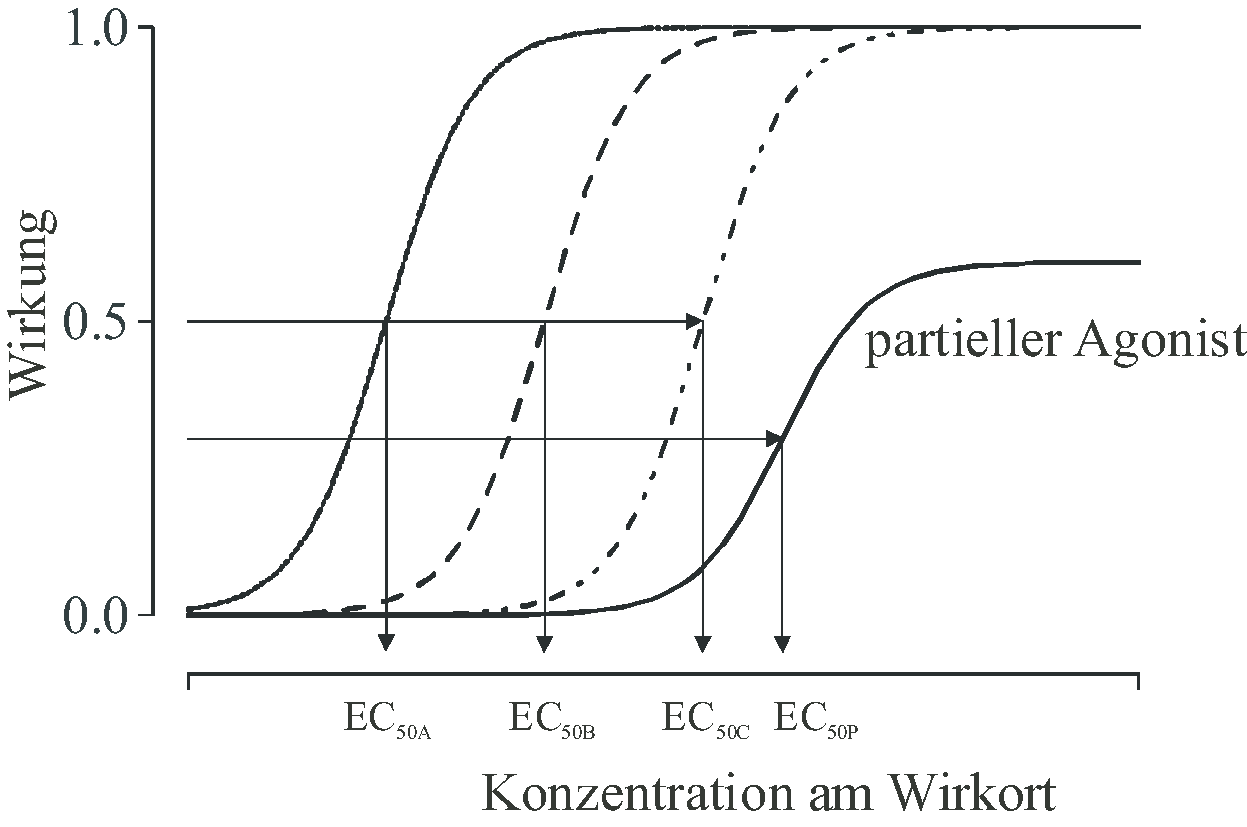
\includegraphics[clip=true,width=0.8\textwidth]{./pd2.pdf}
}
\mode<article>{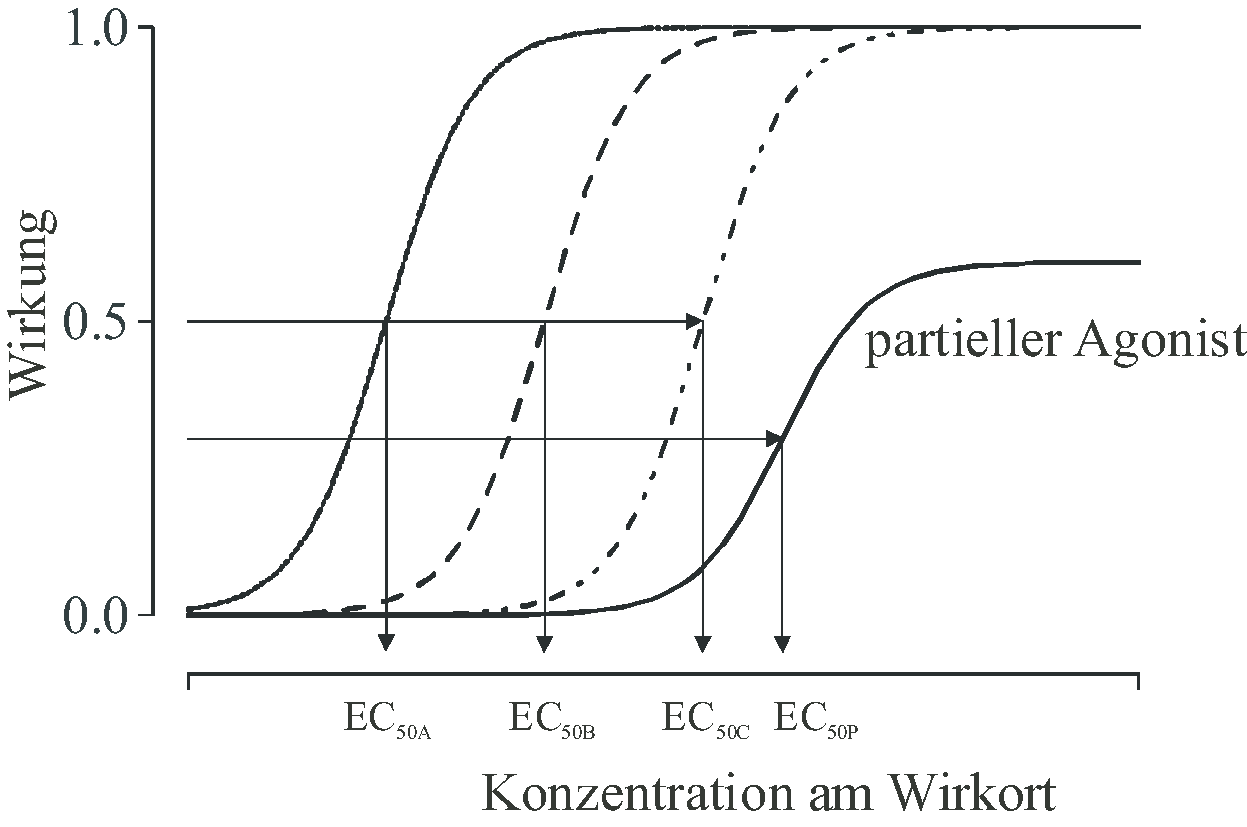
\includegraphics[clip=true,width=0.7\textwidth]{./pd2.pdf}
}

\note<1>{
Alle Begriffe erkl�ren.\\
Die Steigung ebenfalls einzeichnen.\\


Agonist und Antagonist haben eine ganz andere Wirkung am
Rezeptor. Agonist bindet sich und entfaltet eine Wirkung. Der
Antagonist bindet sich an den Receptor und bewirkt nichts. Falls
eine gewisse (partielle) Wirkung entfaltet wird spricht man von
einem partiellen Agonisten. }
\end{block}
}





\mode<article>{\pagebreak}
\subsection{PD und Elimination}
\mode<all>
\mode*

\subsection{Elimination, Relevanter Konzentrationsabfall}


\frame{
\mode<presentation>{
\begin{tikzpicture}[remember picture, overlay]
\node[inner sep=0pt,xshift=0cm] at (current page.center){
\tikz \draw[step=2mm,black!50] (0,0) grid (126mm,94mm);
};
{
\node[coordinate] at (1cm,-3.55cm) (start) {};
\node[coordinate] at (1cm,3cm) (end) {};
\node[coordinate] at (10cm,-3.55cm) (endy) {};
\draw[->,thick] (start)--(end);
\draw[->,thick] (start)--(endy);
};
\end{tikzpicture}
}
\frametitle{Klinisch relevanter Konzentrationsabfall}
\note<1>{
\begin{itemize}
\item
Sigmoide Kurve: Keine fixe Konzentration, keine fixe Zeit: Wenn Konzentration um 70\% abfallen muss damit Patient z.B. erwacht, dann ist diese Zeit relevant.
\item
Excel Simulation - Vergleich von verschiedenen Kurven.
\end{itemize}
}
\infina
}


\mode<article>{
\vspace{1cm}

\begin{tikzpicture}[auto]
\node[inner sep=0pt,xshift=0cm] at (current page.center){
\tikz \draw[step=2mm,black!50] (0,0) grid (140mm,70mm);
};
\end{tikzpicture}

\vspace{0.5cm}
Um abzusch�tzen, wie lange es nach abstellen der Medikamentenzufuhr geht, bis die Wirkung \enquote{weg ist} muss man wissen, wieviel die Konzentration absinken muss. Es gibt keinen Grund anzunehmen, dass f�r die verschiedenen Wirkungen der An�sthetika, ein Abfall der Konzentration auf die H�lfte (\HWZ !) klinisch klinisch relevant ist. F�r volatile An�sthetika braucht es Reduktion der Konzentration um ca. 70 - 80 \% damit ein Patient erwacht. (ad�quate An�sthesie bis Erwachen). Eine �hnliche Gr�ssenordnung ist auch f�r Propofol beschrieben. 



}



\mode<article>{\pagebreak}
\mode<all>
\section{Wirkortkonzentration}
\mode<all>
% !TEX root = ./pkMain.tex
\mode*

Lange Zeit nahm man an, dass man aufgrund der Konzentration eines Medikamentes im Blut, die Wirkung absch�tzen kann. Von der intraven�sen Injektion erwartete man resp. man nahm an, dass die Wirkung sofort eintreten w�rde.

\begin{frame}<presentation>[label=ZeitBez]
\begin{tikzpicture}[remember picture, overlay]
\node[inner sep=0pt,xshift=0cm] at (current page.center){
\tikz \draw[step=2mm,black!50] (0,0) grid (126mm,94mm);
};
{
\node[coordinate] at (1cm,-3.55cm) (start) {};
\node[coordinate] at (1cm,3cm) (end) {};
\node[coordinate] at (10cm,-3.55cm) (endy) {};
\draw[->,thick] (start)--(end);
\draw[->,thick] (start)--(endy);
};
\end{tikzpicture}

\frametitle{Zeitliche Beziehung: Plasma Konzentration $\Leftrightarrow$ Wirkung}
\note<1>{
\begin{itemize}
\item
Bolus Gabe
\item
Darstellen, dass Konzentration zu Beginn hoch, Wirkung tief.
\item
Dieselbe Wirkung bei verschiedenen Konzentrationen
\item
Keine eindeutige Beziehung zw. Konzentration und Wirkung.
\item
Infusion: Verlauf er Konzentration\\
Um so weniger zwischen Infusionsrate und Wirkung
\end{itemize}
}
\infina
\end{frame}

\mode<article>{
\begin{center}
\includeslide[width=0.8\textwidth]{ZeitBez}
\end{center}
}


\begin{frame}
\frametitle{Konzentration am Wirkort}
\begin{itemize}[<+->]
\item
Die Blutkonzentration hat keine direkte Beziehung zur wirkung
\item
Das Medikamente am Wirkort (Wirkortkonzentration) ist verantwortlich f�r Wirkung
\item
Im \enquote{Steady State} sind Konzentration im Blut und Wirkort Konzentration gleich.
\item
Die Wirkortkonzentration steigt und f\"allt entsprechend dem Konzentrationsgradienten. ($=$ Unterschied der Konzentrationen)
\end{itemize}
\note<1>{
\begin{itemize}
\item
Mit Cylinder das Effect Kompartiment zeigen.
\item
Simulation mit einem Bolus
\item
Simulation mit konstanter Infusion
\item
Simulation die zeigt, dass mit Bolus die Plasmakonzentration \enquote{\"uberschossen} werden muss.
\end{itemize}
}
\infina
\end{frame}


\mode<article>{Bei der Beschreibung der Pharmakokinetik wurde auf die
Konzentration des Medikamentes im Blut resp. Plasma Bezug genommen. Die
An�sthetika entfalten ihre Wirkung aber nicht im direkt im Blut in einem
anderen Kompartiment z.B. im Gehirn. Es braucht aber Zeit bis das
Medikament vom Blut in dieses Kompartiment aufgenommen ist. Es gibt also
ein weiteres Kompartiment, den Wirkort, das wir in unsere �berlegungen
einbeziehen m�ssen.}


\frame{
\frametitle{Input, Konzentration, Wirkung}
\mode<presentation>{
\begin{center}
    \includegraphics<1>[clip=true,width=0.9\textwidth]{./receptor/receptorOn1.png}
    \includegraphics<2>[clip=true,width=0.9\textwidth]{./receptor/receptorOn2.png}
    \includegraphics<3>[clip=true,width=0.9\textwidth]{./receptor/receptorOn3.png}
    \includegraphics<4>[clip=true,width=0.9\textwidth]{./receptor/receptorOn4.png}
    \includegraphics<5>[clip=true,width=0.9\textwidth]{./receptor/receptorOn5a.png}
    \includegraphics<6>[clip=true,width=0.9\textwidth]{./receptor/receptorOn5.png}
\end{center}
}

\mode<article>{
\centering
\begin{figure}[H]
    \includegraphics<1>[clip=true,width=0.3\textwidth]{./receptor/receptorOn3.png}
\caption{Es braucht Zeit bis sich die Wirkung, die mit einer bestimmten
Plasmakonzentration korreliert sich etabliert hat. Initial hohe Konzentration im Blut, das
Medikament hat den Rezeptor noch nicht erreicht}
\end{figure}
}
\note<1>{.}
}


\frame{
\frametitle{Wirkverlust $\Leftarrow$ Konzentration}
\mode<presentation>{
\begin{center}
    \includegraphics<1>[clip=true,width=0.9\textwidth]{./receptor/receptorOff1.png}
    \includegraphics<2>[clip=true,width=0.9\textwidth]{./receptor/receptorOff2.png}
    \includegraphics<3>[clip=true,width=0.9\textwidth]{./receptor/receptorOff3.png}
    \includegraphics<4>[clip=true,width=0.9\textwidth]{./receptor/receptorOff4.png}
    \includegraphics<5>[clip=true,width=0.9\textwidth]{./receptor/receptorOff5.png}
    \includegraphics<6>[clip=true,width=0.9\textwidth]{./receptor/receptorOff6.png}
    \includegraphics<7>[clip=true,width=0.9\textwidth]{./receptor/receptorOff7.png}
\end{center}
}
\mode<article>{
\centering
\begin{figure}[H]
    \includegraphics<1>[clip=true,width=0.3\textwidth]{./receptor/receptorOff3.png}
\caption{Die Konzentration im BLut sinkt. Dadurch entsteht ein umgekehrter Konzentrationsgradient.}
\end{figure}
}
\note<1>{.}
}








\subsection{$t_{peak}$}


\begin{frame}<presentation>[label=PeakNachBolus]
\begin{tikzpicture}[remember picture, overlay]
\node[inner sep=0pt,xshift=0cm] at (current page.center){
\tikz \draw[step=2mm,black!50] (0,0) grid (126mm,94mm);
};
{
\node[coordinate] at (1cm,-3.55cm) (start) {};
\node[coordinate] at (1cm,3cm) (end) {};
\node[coordinate] at (10cm,-3.55cm) (endy) {};
\draw[->,thick] (start)--(end);
\draw[->,thick] (start)--(endy);
};
\end{tikzpicture}

\frametitle{Maximale Konzentration nach Bolus \enquote{Peak} Konzentration}
\note<1>{
\begin{itemize}
\item
Kurve f\"ur Bolus  - $C_{e}$
\item
Zeigen der $t_{peak}$; Wenn Bolus verdoppelt wie lange geht es bis maximale Konzentration erreicht?
\item
Zeigen, dass mit doppeltem Bolus, gleiche Kurve aber doppelt so hoch
\item
Ist der Wirkeintritt bei Verdoppelung der Konzentration schneller? (Esmeron)
\item
Zeigen, dass Wirkeintritt, definiert als Zeit bis zu einer Konzentration schneller.
\item
Noch einmal mit Cylinders zeigen
\item
FentanaBolus.xls
\end{itemize}
}
\infina
\end{frame}

\mode<article>{
\begin{center}
    \includeslide[width=0.8\textwidth]{PeakNachBolus}
\end{center}
}

Nach dem Verabreichen eines Bolus eines An�sthetikums f�llt die initial hohe Konzentration im Blut ab und die Konzentration am Wirkort steigt auf Grund des Konzentrationsgradienten an. Wenn die Konzentration am Wirkort und die Konzentration im Blut gleich sind, ist die Konzentration am Wirkort maximal. Die Zeit bis diese maximale Konzentration erreicht wird ist unabh�ngig von der Gr�sse des Bolus gleich!


Warum verabreichen wir eine h�here Dosis des Nicht-Depolarisierenden Muskelrelaxans bei einer Notfalleinleitung?

\frame<presentation>[label=ZeitWirkung]{
\begin{tikzpicture}[remember picture, overlay]
\node[inner sep=0pt,xshift=0cm] at (current page.center){
\tikz \draw[step=2mm,black!50] (0,0) grid (126mm,94mm);
};
{
\node[coordinate] at (1cm,-3.55cm) (start) {};
\node[coordinate] at (1cm,3cm) (end) {};
\node[coordinate] at (10cm,-3.55cm) (endy) {};
\draw[->,thick] (start)--(end);
\draw[->,thick] (start)--(endy);
};
\end{tikzpicture}

\frametitle{Zeit $\Leftrightarrow$ Wirkung: Erh\"ohung der Dosis}
\note<1>{
\begin{itemize}
\item
Submaximale Konzentration mit geringen Bolus
\item
Zweite submaximale Dosis
\item
Dritte supramaximale Dosis
\item
Vierte supramaximale Dosis: Maximale Wirkung gleich: $t_{peak}$ nicht erkennbar.
\item
Zusammenfassen: Mit derselben Infusionsrate k\"onnen die Konzentrationen verschieden sein. F\"ur die $C_{e}$  gilt dies sogar noch mehr. (RiseToSS.xls zeigt den Verlauf bei konstanter Infusion.)
\end{itemize}
}
\infina
}

\mode<article>{
\begin{center}
\includeslide[width=0.8\textwidth]{ZeitWirkung}
\end{center}
}


\mode<article>{
\vspace{0.5cm}
\begin{minipage}{\textwidth}
}

\begin{frame}
\frametitle{T peak, Pentothal}
\begin{center}
\includegraphics[width=0.6\textwidth]{../Figures/FlaishonPentoBIS1997.jpg}
\end{center}
\note<1>{.}
\end{frame}

\mode<article>{
\end{minipage}
}

\mode<article>{
\begin{minipage}{\textwidth}
}

\begin{frame}
\frametitle{T peak, Propofol}
\begin{center}
\includegraphics[width=0.6\textwidth]{../Figures/FlaishonPropofolBIS1997.jpg}
\end{center}
\note<1>{.}
\end{frame}

\mode<article>{

Obwohl Propofol eine \enquote{schnellere} Kinetik hat, dauert es nach einer �quipotenten potenten Dosis l�nger bis ein Patient aufwacht als nach Thiopental
\vspace{.5cm}
\end{minipage}
}

\mode<article>{
\begin{minipage}{\textwidth}
}

\begin{frame}
\frametitle{T peak, Etomidate versus Propofol}
\begin{center}
\includegraphics[width=0.6\textwidth]{../Figures/EtomidatePropofolTPeak.jpg}
\end{center}
\note<1>{.}
\end{frame}

\mode<article>{
Mit Etomidate wird der maximale Effekt nach einer Bolus Dosis schneller erreicht als nach Gabe von Propofol.

\end{minipage}
}


\mode<article>{\pagebreak}
\section{Pharmakokinetische Modelle}
\mode<all>
% !TEX root = ./pkMain.tex
\mode*


\begin{frame}
\frametitle{Kompartiment Modelle: Abstraktion}

\note<1>{
\begin{itemize}
\item
Zeichne: Pictogramm Mensch: Spritze: Injektion $\Rightarrow$ xy Grafik mit Konzentrationsverlauf.
\item
Es gibt Formeln die Kurven ergeben. (z.B. $C = (Dosis * Gewicht)^{t}$)
\item
Formel kann nicht jede Form haben da: z.B. Konzentration f\"allt ab, Abfall abh\"angig von Konzentration etc.
\item
Was abl\"auft bei der graphischen Darstellung kann als Formel ausgedr\"uckt werden.
\end{itemize}
}
\end{frame}

%: PK Studie

\frame{ \begin{exampleblock}{Ablauf einer PK Studie:}
     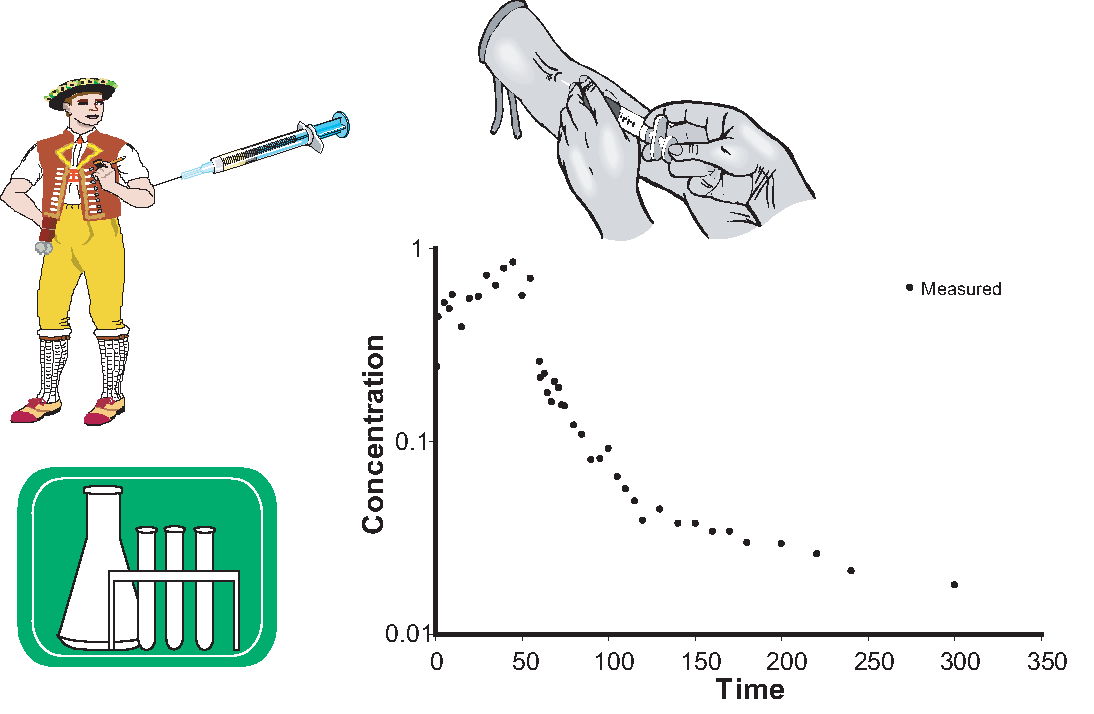
\includegraphics[clip=true,width=\textwidth]{PKStudy.pdf}
\end{exampleblock}
\note<1>{
\begin{itemize}
\item
Ablauf zeigen: Menschen, mehrere Individuen
\item
In die Grafik zeichnen.
\end{itemize}}
}


\frame{
\begin{alertblock}{Herleitung von PK Modellen basiert auf:}
    \begin{itemize}
        \item Bekanntem Input (z.B. meist eine konstante Infusion) und gemessenen Konzentrationen
        \item Nichtlinearer Regression zu Bestimmung der Modellparameter: $V_1$,$V_2$,$V_3$,$Cl_1$,$Cl_2$,$Cl_3$
    \end{itemize}
    \begin{center}
        \href{run:Fitsimulation.xls}{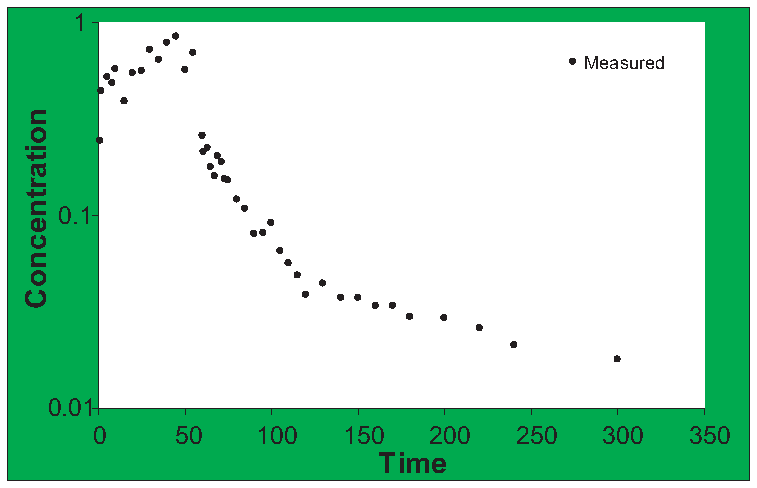
\includegraphics[width=8cm]{ForFitSim.pdf}}
    \end{center}
\end{alertblock}
\note<1>{ Beachte den Text im Manuskript.\\
Bei der Simulation die verschiedenen Parameter ver�ndern und auf die
Ver�nderung der Kurve aufmerksam machen.\\
Die Sch�ler sollen die Kurve durch die Datenpunkte im Manuskript
einzeichnen.}
}


\begin{frame}
\frametitle{Individualisieren!}
\begin{itemize}[<+->]
\item Es m�ssen viele \enquote{verschiedene} Patientengruppen untersucht werden. (m/f, dick/d�nn, alt/jung)
\item Die Unterschiede zwischen den einzelnen untersuchten Patienten m�ssen gesucht werden
\item F�r jeden zuk�nftgen Patienten k�nnen dann  mit dem Modell die passenden Parameter berechnet werden. (siehe Eingabe in TCI)
\end{itemize}
\note<1>{}
\infina
\end{frame}



\mode<article>{\pagebreak}
\section{Verwendung der Modelle: TCI}
\mode<all>
% !TEX root = ./pkMain.tex
\mode*

\begin{frame}
\frametitle{Verwendung der Modelle}
\begin{itemize}[<+->]
\item
Dosierungsempfehlungen ausarbeiten.
\item
Extrapolieren - Interpolieren
\item
Simulieren
\item
In Computer einbauen: Computer kontrollierte Infusion (Target Controlled Infusion)
\end{itemize}
\note<1>{
\begin{itemize}
\item
Aufgrund der Modelle entstanden die Empfehlungen f\"ur Remifentanil
\item
Extrapolieren gef\"ahrlich. Adip\"ose - Alter
\item
Zeigen: Wie sieht Roberts Schema aus
\item
Mit Cylinder zeigen was bei TCI passiert.
\end{itemize}}
\infina
\end{frame}



\mode<article>{\pagebreak}

{\huge{2. Teil Pharmakokinetik, Pharmakodynamik}}

\section*{}
\vspace{4cm}
\begin{frame}
\frametitle{Themen aus den ersten 4 Stunden.}
\begin{itemize}[<+->]
	\item Warum m\"ussen sie bei \"alteren Patienten die Zufuhr der An\"asthetika (im Vergleich zu j\"ungeren) anpassen?
	\item Zeichen sie den Verlauf der Konzentration von Propofol bei konstanter Infusion (z.B. 6 $\frac{\text{mg}}{\text{kg h}}$).
	\item Erkl\"aren sie den Verlauf der Kurve aufgrund von Begriffen wie Clearance resp. Eliminationsrate. 
	\vspace{1cm}
	\item Was ist \enquote{Kontext sensitive Halbwertszeit}?
	\item Wie kann es ein, dass ein gr\"osserer Bolus eines Medikamentes (z.B. Rocuronium) den \enquote{Wirkeintritt} nicht aber die Zeit zur maximalen Wirkung beeinflusst?
\end{itemize}
\note<1>{
\begin{itemize}
	\item Kinetik und Empfindlichkeit.
	\item Zeitachse und Konzentration - erst nach einer Viertelstunde. 
	\item Die Zufuhr ist konstant, die Eliminationsrate nimmt zu bis  $C_{ss}$.
	\item Abh\"angigkeit von der Dauer der Zufuhr
	\item Die Wirkung wird weit gr\"osser!    
\end{itemize}
}
\infina
\end{frame}


\mode<article>{\pagebreak}
\section{An\"asthetika (im engeren Sinne)}
\subsection{i.v. Hypnotika}
\mode<all>
% !TEX root = ./pkMain.tex
\mode*

\begin{frame}<1>[label=hypno]
\frametitle{Gebr�uchliche Hypnotika f�r i.v. An�sthesie}
\begin{itemize}[<+->]
\item
Propofol
\item
Thiopental
\item
Etomidate
\item
Midazolam
\item
Ketamin
\item
Dexmedetomidine
\end{itemize}

\note<1>{
\begin{itemize}
	\item
	Propofol
	\item
	.
\end{itemize}
}
\infina
\end{frame}

\mode<all>
\mode*

\begin{frame}
\frametitle{Propofol (Di-isopropylphenol)}
\begin{itemize}[<+->]
\item
Vasodilatation - Ausgepr�gter Blutdruckbafall (bei alten und hypovol�men Patienten)
\item
Angenehmer Schlaf - \enquote{angenehme Tr�ume}
\item
antiemetische Wirkung (wenn f�r Unterhalt der An�sthesie gebraucht.)
\item
antipruritisch
\item
Propofol - Infusionssyndrom (Metabolische Azidose, Herzversagen, akute Niereninsuffizienz, Rhabdomyolyse), vor allem bei Kleinkindern und bei Verabreichung �ber lange Zeit in hohen Infusionsraten beschrieben. Wenn nicht erkannt, Verlauf t�dlich! 
\item
In Fett Emulsion (Sojabohnen�l) gel�st.
\item
Allergy gegen Soja oder Eier keine Kontraindikation
\item
Wird auch w�hrend Schwangerschaft und f�r Sectio eingesetzt

\item
Verschiedene Galeniken! (Na-EDTA, Bisulfit)
\end{itemize}
\note<1>{
\begin{itemize}
\item
.\end{itemize}
}
\infina
\end{frame}



\againframe<2>{hypno}

\mode<all>
% !TEX root = ./pkMain.tex
\mode*

\begin{frame}
\frametitle{Thiopental}
\begin{itemize}[<+->]
\item
Negativ inotrop (weniger Afterload Senkung als Propofol)
\item
Gute antikonvulsive Eigenschaft (schon 25 - 50 mg)
\item
Reduziert Hirn-Metabolismus
\item
Kurze Wirkung nach einer Einzeldosis
\item
Langsame terminale Elimination
\item
F�r kontinuierliche Gabe nicht geeignet
\item
Gefahr der Gef�sssch�digung bei intraarterieller Injektion
\item
Kontraindiziert bei Porphyrie
\end{itemize}
\note<1>{
\begin{itemize}
\item
Stimulation der Amino Laevulin S�ure Synthase - Beginn der H�m Synthese stimuliert!
\end{itemize}
}
\infina
\end{frame}



\againframe<3>{hypno}

\mode<all>
% !TEX root = ./pkMain.tex
\mode*

\begin{frame}
\frametitle{Etomidate}
\begin{itemize}[<+->]
\item
Sehr gute h�modynamische Stabilit�t
\item
Kann schon nach einer Dosis zu einer NN-Insuffizienz f�hren.
(H�modynamik!)
\item
Durch Gabe von Steroiden (zT.) behandelbar
\item
Kann bei Einleitung zu Myoklonus f�hren
\item
Wenig Atemdepression
\item
Umstritten bei kritisch Kranken (insbesondere Sepsis): Erh�hte Mortalit�t - Unbeeinflusst von Steroid Substitution
\end{itemize}
\note<1>{
\begin{itemize}
\item
Es wird ein Enzym - 11$\beta$-Hydroxylase - und damit die Nebenniere gehemmt
.\end{itemize}
}
\infina
\end{frame}



\againframe<4>{hypno}

\mode<all>
\mode*

\begin{frame}
\frametitle{Midazolam}
\begin{itemize}[<+->]
\item
H�modynamisch stabil
\item
Langsamer Wirkeintritt
\item
Kann mit Flumazenil antagonisiert werden
\end{itemize}
\note<1>{
\begin{itemize}
\item
.\end{itemize}
}
\infina
\end{frame}



\againframe<4>{hypno}

\mode<all>
\mode*

\begin{frame}
\frametitle{Ketamin}
\begin{itemize}[<+->]
\item
Erh�ht Sympathikotonus und setzt Katecholamine aus Neben Niere frei. H�modynamisch sehr stabil!
\item
Bewirkt Bronchodilatation
\item
Wirkt analgetisch (NMDA Rezeptor)
\item
Kann auch intramuscul�r gegeben werden
\item
Halluzinationen und (Alb)Tr�ume realtiv h�ufig (Benzodiazepine, Propofol)
\end{itemize}

\note<1>{
\begin{itemize}
\item .
\end{itemize}
}
\infina
\end{frame}



\againframe<4>{hypno}

\mode<all>
\mode*

\begin{frame}
\frametitle{Dexmedetomidine}
\begin{itemize}[<+->]
\item
$\alpha^{2}$ Agonist
\item
Induziert \enquote{Schlaf} aus dem Patienten weckbar. (Wirkung via Locus coeruleus)
\item
Kann Bradykardie bewirken: Zentrale Sympathikolyse $+$ Baroreflex (Bolusgabe!)
\item
Bei Bolusgabe direkte periphere $\alpha$ Rezeptoren bedingte Vasokonstriktion mit (kurzzeitiger) Hypertonie m�glich.
\item
Zulassung f�r Sedation auf der Intensivstation und prozedurale - Wachsedierung bei Erwachsenen > 18 J
\end{itemize}

\note<1>{
\begin{itemize}
\item .
\end{itemize}
}
\infina
\end{frame}





\mode<article>{\pagebreak}
\subsection{i.v. Opiate}
\mode<all>
% !TEX root = ./pkMain.tex
\mode*

\begin{frame}<1>[label=opiate]
\frametitle{Gebr�uchliche Opiate}
\begin{itemize}[<+->]
\item
Fentanyl
\item
Remifentanil
\item
Alfentanil
\item
Pethidin
\end{itemize}
\note<1>{
\begin{itemize}
\item
-
\item
.
\end{itemize}
}
\infina
\end{frame}

\mode<all>
% !TEX root = ./pkMain.tex
\mode*

\begin{frame}
\frametitle{Fentanyl}
\begin{itemize}[<+->]
\item
$\mu$ Agonist
\item
$t_{peak}$ ca. 3.5 min.
\item
terminale Halbwertszeit: $ > 7 h$
\item 
Potenz: (50)
\end{itemize}
\note<1>{
\begin{itemize}
\item
.\end{itemize}
}
\infina
\end{frame}



\againframe<2>{opiate}

\mode<all>
% !TEX root = ./pkMain.tex
\mode*

\begin{frame}
\frametitle{Remifentanil}
\begin{itemize}[<+->]
\item
$\mu$ Agonist
\item
Direkte vasodilatierende Wirkung
\item
Wird durch Esterasen metabolisiert (nicht spezifische)
\item
Schneller Wirkeintritt: ($t_{peak} \approx 1.5 min.$)
\item
Kinetisch in \enquote{separater Liga} - Sehr schnelle Elimination!
\item 
Potenz: (40)
\end{itemize}
\note<1>{
\begin{itemize}
\item
.\end{itemize}
}
\infina
\end{frame}




\againframe<3>{opiate}

\mode<all>
% !TEX root = ./pkMain.tex
\mode*

\begin{frame}
\frametitle{Alfentanil}
\begin{itemize}[<+->]
\item
$\mu$ Agonist
\item
Schneller Wirkeintritt: ($t_{peak} \approx 1.5 min.$)
\item
Bis 1 h Zufuhr, Elimination �hnlich Fentanyl
\item
Lange Infusionsdauer: CSHT ca. 50 min
\item
K\"onnte h�ufiger eingesetzt werden!
\item 
Potenz: (1)
\end{itemize}
\note<1>{
\begin{itemize}
\item
.\end{itemize}
}
\infina
\end{frame}



\againframe<4>{opiate}

\mode<all>
% !TEX root = ./pkMain.tex
\mode*
\begin{frame}
\frametitle{Pethidin}
\begin{itemize}[<+->]
\item
Hat strukturelle �hnlichkeit mit Atropin. (Macht keine Miose)
\item
Bei Shivering. (25 mg)
\item
Metabolit Nor-Pethidine ist toxisch (Kr�mpfe); Pethidin nicht �ber l�ngere Zeit verabreichen. Maximaldosis/24 ca. 600 mg!
\item
Einziges cardio depressives Opiat!
\end{itemize}
\note<1>{
\begin{itemize}
\item Gr\"ossere Mengen sollten nicht gegeben werden.
\item Wird zuviel eingesetzt!
\item Indiziert bei Shivering
\end{itemize}
}
\infina
\end{frame}






\mode<article>{\pagebreak}
\section{Praxis der TIVA}
\mode<all>
% !TEX root = ./pkBeamer.tex
\mode*


\mode<all>{

\subsection{i.v. An�sthesie mit TCI}


\begin{frame}
\frametitle{Indikation \mode<presentation>{f�r \subsecname}}
\begin{itemize}
\item
  grunds�tzlich immer m�glich
\item
  bei hohem Risiko f�r PONV
\item
  bei maligner Hyperthermie
\item
  um Umgebungskontamination mit Volatilen zu verhindern
\item
  bei Neuromonitoring mit evozierten Potentialen
\item
  wenn nichthypnotische Eigenschaften von Propofol erw�nscht sind
\end{itemize}
\note<1>{.}
\end{frame}


\begin{frame}
\frametitle{Kontraindikationen \mode<presentation>{f�r \subsecname}}
\begin{itemize}
\item
  Absolut: Allergie gegen Propofol oder Remifentanil
\item
  Relativ: Hypovol�mie, Kreislaufinstabilit�t, Venenpunktionsstelle
  nicht einsehbar
\end{itemize}
\note<1>{.}
\end{frame}


\begin{frame}
\frametitle{Prinzip der An�sthesief�hrung mit TCI}
\begin{itemize}
\item
  mit Propofol sicherstellen, dass der Patient schl�ft.
\item
  mit Remifentanil (und Fentanyl) die schmerzbedingte Kreislaufreaktion
  behandeln
\item
  Hohe Opiat-Konzentrationen reduzieren die Wahrscheinlichkeit von
  motorischen Reaktionen auf Stimuli. (auch bei tiefen Konzentrationen
  von Propofol)
\item
  Gegen Ende der An�sthesie wird unter Ber�cksichtigung der 70\%
  Konzentrationsabfall -Zeit (bezieht sich auf durchschnittliche
  intraoperative Konzentration.) Propofol rechtzeitig abgestellt.
  Gleichzeitig wird die Remifentanil Konzentration kontinuierlich erh�ht
  (verhindern mot. Reaktionen)
\end{itemize}
\note<1>{.}
\end{frame}


\begin{frame}
\frametitle{Dosierung / Zielkonzentrationen Propofol}
\begin{itemize}
\item
  grunds�tzlich die Wirkung eintitrieren $\Rightarrow$ sehr vorsichtig
  bei �lteren Patienten
 \item
   Bei Patienten \textgreater{} 65 Jahre (biologisch) mit $2 \mu g/ml$
   Wirkortkonzentration ($C_e$) beginnen (entspricht ca. 0.5 mg Bolus). Warten bis
   $C_e$ erreicht, erst dann Konzentration
   erh�hen
\item
  Junge Patienten brauchen f�r Einlage der LM oft relativ hohe
  Konzentrationen von Propofol (6--8 $\mu g/ml$)
\item
  Intraoperative Propofolgabe gem�ss BIS (40--60) oder klinischen
  Zeichen der Wachheit (in erster Linie Reaktion auf Ansprechen)
\end{itemize}
\note<1>{.}
\end{frame}


\begin{frame}
\frametitle{Dosierung / Zielkonzentrationen, Remifentanil - Fentanyl}
\begin{itemize}
\item
  vor Einleitung 200 $\mu g$ Fentanyl (alte Patienten, kurze Eingriffe: Dosis
  reduzieren)
\item
  f�r kurze Eingriffe \textless{} 1--2 h kein zus�tzliches Fentanyl vor
  Schnitt
\item
  f�r Eingriff \textgreater{} 1--2 h in der Regel 100 - 200 $\mu g$ Fentanyl
  zus�tzlich vor Schnitt.
\item
  bei langen Operationen zu Beginn Kreislaufreaktionen (Hypertension,
  Tachykardie) mit Fentanyl behandeln (bei bariatrischen Eingriffen 1
  mg w�hrend ersten 45 min m�glich)
\item
  KEIN Fentanyl mehr 1--2 h vor Ende der Operation! - grunds�tzlich
  Fentanyl nur zu Beginn
  Intraoperativ abnehmende Fentanyl Wirkung mit Remifentanil
  kompensieren (Intraoperativ bis ca. 4--6 ng /ml); Gegen Ende der
  Operation v.a. wenn Propofol gestoppt ist, Zielkonzentration bis
  \textgreater{} 10 ng/ml. Stoppen der Infusion, wenn Haut geschlossen.
\end{itemize}
\note<1>{.}
\end{frame}




}

\mode<all>{
% !TEX root = ./pkArticle.tex
\subsection{i.v. Applikation: TIVA / TCI}

\begin{frame} 
\frametitle{Material  \mode<presentation>{- \emph{\subsecname}}}
\begin{itemize}
\item
 i.v. Set (verschiedene Anbieter) f�r 2 Medikamente
\item
R�ckschlagventile
\item
Dreiwegehahn
\item
D�nne Infusionsverl�ngerungen. 
\end{itemize}

 \note<1>{ 
\begin{itemize}
   \item Wenn kein spezielles Set vorhanden, sollte immer gleich vorgegangen werden - gleiche Verl�ngerungen, gleich zusammen gesetzt.
   \item R�ckschlagventile sind m.E. ein Muss!
   \item Compliance der Verl�ngerungen. 
\end{itemize}

\bf{Photo resp. Zeichnung}
}
\end{frame}


\begin{frame} 
\frametitle{Grunds�tze  \mode<presentation>{- \emph{\subsecname}}}
\begin{itemize}
\item
  Totraum immer so klein wie m�glich halten! (Totraum: von Spitze der
  Venenkan�le bis Verbindung mit Leitung f�r Medikament.) Wenn Verl�ngerung notwendig: D�nne, m�glichst kurze Verl�ngerung!
\item
  Zufuhr immer gegen das Zur�cklaufen sichern (R�ckschlagventile!)
\item
  Wenn \it{zentrale} Leitung vorhanden, alle kontinuierlichen Medikamente via
  ZVK verabreichen
\end{itemize}
\note<1>{Zeichnen eines Systems! Venflon - Evt. kurze Verl�ngerung = Flexibilit�t, Zufuhr der zwei Medikamente, Absicherung des zur�ckfliessens - Gegenseitiges zur�ckfliessen bei zwei Medikamenten.\newline
Bedeutung der Tr�gerl�sung. \bf{Zeichung}
}
\end{frame}


\begin{frame} 
\frametitle{Ven�ser Zugang  \mode<presentation>{- \emph{\subsecname}}}
\begin{itemize}
  \item 
  In der Regel peripherer Zugang (16 G) (oder ZVK)
  \item 
  Leitungen von Abteilung nur in Ausnahmef�llen weiter benutzen
  \item 
  Leitung muss sicher laufen und die Venflon Punktionsstelle w�hrend Betrieb eingesehen werden k�nnen resp. sichtbar gemacht werden k�nnen.
\end{itemize}

\note<1>{
\begin{itemize}
  \item 
  Bedeutung des i.v. Zugangs: keine Monitoring!
  \item 
  Kann jederzeit \enquote{unterbrochen} werden.
  \item 
  Sicht auf Leitung extrem wichtig! (fehlen ist m.E. relative KI) \bf{Photo}
\end{itemize}
}
\end{frame}


\begin{frame} 
\frametitle{Vorbereiten TCI Pumpe (Base Primea)}
\begin{enumerate}
\item
  In zwei 50ml Spritzen Propofol 1 \%, Remifentanil (z.B.) $40 \frac{\mu g}{ml}$ (50 ml)
\mode<article>{\vspace{.1cm}\newline Je verd�nnter die Medikamente desto kleiner die Auswirkung bei Verwechslung. Bei TCI Systemen sollte bei \enquote{vern�nftiger} Zielkonzentration eines Medikamentes auch bei Verwechslung der Spritzen keine den Patienten gef�hrdende Menge des \enquote{falschen} Medikamentes verabreicht werden.}
\item
  Ganzes Set luftfrei machen.
\item
  Propofol Spritze in die unterste Spritzenpumpe einspannen (Sitz der
  Spritze �berpr�fen)
\item
  Remifentanil Spritze in die zweitunterste Spritzenpumpe einspannen.
  (Sitz der Spritze �berpr�fen)\mode<article>{\vspace{.1cm}\newline Pumpen arbeiten oft \enquote{interaktiv}. Bei der Bedienung nie einfach \enquote{durchklicken}! Man kann einmal zuviel klicken (Pumpe l�uft dann unbeabsichtigt) oder einen Warnhinweis �bersehen.  
}   
\item
  Infusionsset anschliessen. Verbindungen auf Dichtigkeit und festen
  Sitz �berpr�fen.
  \mode<article>{\vspace{.1cm}\newline Es kommt immmer wieder vor, dass Leitungen w�hrend der An�sthesie diskonnektieren! Verbindungen immer wieder �berpr�fen!}
\end{enumerate}
\note<1>{
  \begin{itemize}
    \item Bedeutung der Verd�nnung!
  \end{itemize}
}
\end{frame}


\begin{frame} 
\frametitle{Vorgehen TCI Pumpe (Base Primea)}
\mode<article>{\vspace{.1cm}Ablauf bezieht sich auf die Base Primea von Fresenius. Das Vorgehen ist aber bei allen Spritzenpumpen resp. TCI Systemen �hnlich.}
\begin{enumerate}

\item
  Stromkabel (inkl. Erdung) einstecken und Basis Station einschalten
\item
  Eingeben der Patienten Daten. (Absolutes Gewicht); wenn BMI bei
  adip�sen M�nnern \textgreater{} 42 und Frauen \textgreater{} 35,
  Gr�sse so ``korrigieren'' dass BMI \textless{} 42 resp. \textless{} 35
  \mode<article>{\vspace{.1cm}\newline Mit dieser Korrektur ist es m�glich auch bei bariatrischen Eingriffen die TCI zu nutzen. Diese Korrektur ist \enquote{off-label}!\newline Wenn nicht ganz explizit von der Spritzenpumpe anders verlangt, immer das normale Gewicht eingeben. Die meisten (alle) pharmakokinetischen Modelle gehen vom Normalgewicht aus und Berechnen dann abgeleitete Parameter wie BMI, \enquote{lean body mass} etc. wenn n�tig.}
\item
  W�hlen des Modells (Meist Propofol/Remifentanil)
\item
  Best�tigen Propofol, �berpr�fen der eingegebenen Patientendaten und
  unterstes Modul w�hlen. An Spritzenpumpe Spritzengr�sse und
  Medikamente �berpr�fen und best�tigen.
\item
  Dito f�r Remifentanil (Noch einmal Patientenangaben lesen und
  �berpr�fen!)
  \mode<article>{\vspace{.1cm}\newline Es lohnt sich immer diesselbe Anordnung der Spritzenpumpen zu haben. In einer Institution sollten alle gleich vorgehen. Ist besonders von Vorteil, wenn An�sthesien \enquote{�bergeben} werden.}
\end{enumerate}
\note<1>{.}
\end{frame}



\begin{frame} 
\frametitle{Anschliessen und Starten der TCI}
\begin{enumerate}
\item
  Anschliessen der Medikamentenleitung. �berpr�fen ob R�ckschlagventil
  R�ckfluss der Medikamente verhindert. �ffnen des Dreiwege-Hahn
\item
  Blickkontrolle: Dreiwege-Hahn proximal bei Spritzenpumpe (Propofol und
  Remifentanil) - in korrekter Position!
\item
  �bereinstimmung von Angaben auf Basisstation mit eingespannten
  Spritzen (Propofol in unterer Spritzenpumpe und auf dem Display
  unten!)
\item
  W�hlen einer Zielkonzentration und starten.
\item
  Korrekte Funktion �berpr�fen.
  \mode<article>{\vspace{.1cm}\newline Alles noch einmal \enquote{checken}! Systematisch vorgehen. Grunds�tzlich vor dem Starten einer Spritzenpumpe Leitung, Eingaben bei der Pumpe �berpr�fen-}
\end{enumerate}
\note<1>{.}
\end{frame}



\begin{frame} 
\frametitle{Spritzenwechsel}
\begin{enumerate}
\item
  Vorbereitete Spritze luftfrei machen.
\item
  An Spritzenpumpe ``stop'' dr�cken und Alarm unterdr�cken.
  \mode<article>{\vspace{.1cm}\newline Beachten sie, dass es konzeptionell fundamental verschieden ist, ob sie die Spritzenpumpen stoppen oder ob sie eine Zielkonzentration von \enquote{0} w�hlen. Beim Spritzenwechsel wollen sie nicht, dass die Konzentration abf�llt, sie m�ssen aber die Zufuhr unterbrechen. Wenn die Zufuhr f�r eine gewisse Zeit unterbrochen, wird dies einen Alarm triggern!\newline
  Dasselbe gilt auch wenn sie aus einem Grund die Leitung an eine andere Kan�le anschliessen (z.B. von peripher zu zentral)}
\item
  Arm der Pumpe vollst�ndig zur�ckschieben
\item
  Leere Spritze entnehmen, neue Spritze vorsichtig anschliessen (festen
  Sitz der Leitung, sowie Dichtigkeit �berpr�fen), Klappe an
  Spritzenpumpe schliessen und den Arm mit Spritzenstempel in Kontakt
  bringen - auf korrekte Position achten (muss einrasten).
\item
  An Spritzenpumpe Medikament �berpr�fen und best�tigen.
\item
  An Basisstation ``start'' dr�cken.
\end{enumerate}
\note<1>{.}
\end{frame}



\begin{frame} 
\frametitle{An�sthesie Ende   \mode<presentation>{- \emph{\subsecname}}}
\mode<article>{\vspace{.1cm}Zur�cktitrieren wie weiter hinten beschrieben. Wenn beide $\text{Zielkonzentrationen = 0}$ und An�sthesie ausgeleitet werden soll (vor Extubation/Entfernen der
LMA):}
\begin{itemize}
  \item Dreiwegehahn drehen (verschliessen) und Leitung (An�sthetikazufuhr) diskonnektieren. 
  \item Totraum der verbleibenden Infusionsleitung (kurze Verl�ngerung etc.) mit \textgreater{} 10 ml Infusion sp�len!
\mode<article>{\vspace{.1cm}\newline Je nach Konzentration der Medikamente k�nnen in diesem Totraum relevante Mengen an An�sthetika verbleiben. Wenn Tr�gerl�sung gestoppt oder Infusion aus einem andern Grund nicht l�uft befindet sich unverd�nntes Medikament in der Leitung. Es ist sehr gef�hrlich, wenn diese Menge zu irgendeinem Zeitpunkt \enquote{geflusht} wird. Remifentanil: Gefahr der Apnoe!}

\end{itemize}

\note<1>{.}
\end{frame}


}


\begin{frame}
\frametitle{Technisches}
\begin{itemize}[<+->]
\item Infusionsleitung: Totraum, Kompressionsvolumen
\item Beschriften der Spritzen
\item R�ckschlagventile am richtigen Ort.
\item Infusion im Blickfeld!
\item Vene mit Venflon im Blickfeld!
\item Nach Beenden der Infusion (Medikament im Totraum beachten - leeren!)
\item Druckalarm verstehen!
\item H�henunterschied der Pumpe - hydrostatischer Druck.
\end{itemize}
\note<1>{.}
\infina
\end{frame}







\mode<article>{\pagebreak}
\section{Repetition}
\mode<all>
% !TEX root = ./pkBeamer.tex
\mode*


\begin{frame}
\frametitle{Begriffe die sie nun begriffen haben!}
\begin{itemize}[<+->]
	\item Clearance und $t_{\frac{1}{2}}$: Davon gibt es mehrere f�r unsere Medikamente.
	\item Steady State Konzentration (Beziehung zu Infusionsrate)
	\item Wirkortkonzentration - Verlauf nach einer Bolus Injektion
	\item Pharmakodynamik (Beziehung zwischen der Wirkort Konzentration und Wirkung)
	\item Kontext sensitive \HWZ (und die klinisch wichtige relevante Zeit)
\end{itemize}
\note<1>{.}
\infina
\end{frame}








